%%%%%%%%%%%%%%%%%%%%%%%%%%%%%%%%%%%%%%%%%%%%%%%%%%%%%%%%%%%%%%%%%%%%%
%%%%%%%%%%%%%%%%%%%%%%%%%%%%%%%%%%%%%%%%%%%%%%%%%%%%%%%%%%%%%%%%%%%%%
%%%%%%%%%%%%%%%%%%%%%%%%%%%%%%%%%%%%%%%%%%%%%%%%%%%%%%%%%%%%%%%%%%%%%
\section{Plane curve singularities and the proof of the Main Result}\label{sec:proof_main}

The object of this section is to conclude the proof of the Main Theorem. For that, we now finally specialize to the context of isolated plane curve singularities.

%%%%%%%%%%%%%%%%%%%%%%%%%%%%%%%%%%%%%%%%%%%%%%%%%%%%%%%%%%%%%%%%%%%%%
%%%%%%%%%%%%%%%%%%%%%%%%%%%%%%%%%%%%%%%%%%%%%%%%%%%%%%%%%%%%%%%%%%%%%
\subsection{Plane curve singularities and their integral monodromy modules} In general, we refer to \cite{ACampo1998,ACampo1999,FPST} for the necessary definitions in the study of real Morsifications of plane curve singularities and their divides. That said, we provide here the necessary basic ingredients for our context.\\

Let $(C,0)$ be an isolated plane curve singularity with representative $f:(\C^2,0)\lr(\C,0)$. The Milnor fiber of $f$ will be denoted by $M_f$ and the link of the singularity $(C,0)$ by
$$L(C):=\{(x,y)\in\C^2:f(x,y)=0\}\cap S^3\sse S^3,$$
where $S^3\sse\C^2$ is a 3-sphere of small enough radius, cf.~\cite[Chapter 4]{milnor1968} or \cite[Chapter 4]{Seade19_MilnorFibration}. Note that the intersection of $M_f$ with a 4-ball of that radius is a smoothly embedded surface in a 4-ball bounding $L(C)$. The Milnor fibration provides an explicit model for the geometric monodromy of $(C,0)$, via the fiber bundle
\begin{equation}\label{eq:Milnor_fibration}
\frac{f}{|f|}:S^3\setminus L(C)\lr S^1
\end{equation}
whose fiber is isomorphic to $M_f$, see \cite[Theorem 4.8]{milnor1968}. Specifically, we will focus on the lattice $H_1(M_f;\Z)$ and the action of the geometric monodromy $h\in\pi_0(\mbox{Diff}^c(M_f))$ of \eqref{eq:Milnor_fibration} on $H_1(M_f;\Z)$.

\begin{definition}
Let $(C,0)$ be an isolated plane curve singularity with representative $f:(\C^2,0)\lr(\C,0)$, Milnor fiber $M_f$ and geometric monodromy $h\in\pi_0(\mbox{Diff}^c(M_f))$. By definition, the integral monodromy module of $(C,0)$ is
$$\Z[t,t^{-1}]\circlearrowright H_1(M_f;\Z),\quad t\cdot[\gamma]=h_*([\gamma])$$
where $t$ acts on a cycle in $H_1(M_f;\Z)$ via the induced action
$$h_*:H_1(M_f;\Z)\lr H_1(M_f;\Z).$$
The characteristic polynomial of the monodromy is defined to be $\det(h_*-t\cdot\mbox{Id})$.\hfill$\Box$
\end{definition}

It is a well-known fact, see e.g.~\cite[Section 2]{Durfee1975}, that the Alexander polynomial $\Delta_C(t)$ of the link $L(C)$ of the singularity is the characteristic polynomial of its algebraic monodromy:
\begin{equation}\label{eq:alexander_characteristic_poly}
\Delta_C(t)=\det(t\cdot\mbox{Id}-h_*)
\end{equation}
More generally, the integral monodromy module $\Z[t,t^{-1}]\circlearrowright H_1(M_f;\Z)$ is isomorphic to the Alexander module from \Cref{def:alex-module}:
\begin{equation}\label{eq:alexander_module_monodromy}
A_{L(C)}\cong (H_1(M_f;\Z),h_*)
\end{equation}
as an isomorphism of $\Lambda$-modules, with the covering action on the left hand side, and the algebraic monodromy action on the right hand side. Note that the key isomorphism $H_1(\widetilde{X}_{L(C)};\Z)\cong H_1(M_f;\Z)$ is deduced directly from the fact that the fibers of \eqref{eq:Milnor_fibration} are diffeomorphic to $M_f$ and thus the infinite cover $\widetilde{X}_{L(C)}$ is diffeomorphic to $M_f\times\R$.

\begin{remark}\label{rmk:multivariable_Alexander}
In general, when $L(C)$ has $r$ components, $r\geq2$, there is also the notion of the multi-variable Alexander polynomial $\Delta_{L(C)}^{mv}(t_1,\ldots,t_r)$, see \cite{CDGZ,EisenbudNeumann1985} or \cite{Yamamoto1984} for details on the multi-variable Alexander polynomial of a link. In this manuscript we will not use the multi-variable version beyond noting that the specialization of all $t_i$ variables to be equal to each other yields the identity
$$\det(t\cdot\mbox{Id}-h_*)=(t-1)\Delta_{L(C)}^{mv}(t,\ldots,t),$$
where, by \eqref{eq:alexander_characteristic_poly}, the left hand side can be understood as the one-variable Alexander polynomial.\hfill$\Box$
\end{remark}

Finally, we note that the link of an isolated plane curve singularity is never a split link. Indeed, for two distinct branches $C_i,C_j$ we have the equality:
\begin{equation}\label{eq:linking-intersection}
   \lk(L_i,L_j)=I_0(C_i,C_j)>0,
\end{equation}
where $I_0$ is local intersection multiplicity, cf.~\cite[Chapter~V]{EisenbudNeumann1985} or \cite[Chapters~4\&5]{wall2004}. If a splitting 2-sphere existed, it would partition the components into two nonempty sets and force all linking numbers across the partition to vanish, contradicting \eqref{eq:linking-intersection}. Thus we conclude that an algebraic link is nonsplit, as claimed.\\

\noindent In fact, the entire Alexander module is torsion in the case of algebraic links, as it follows from the existence of the Milnor fibration \cite[Chapter 4]{milnor1968}. Therefore \Cref{prop:dil_module_is_Alexander} implies the following:

\begin{corollary}\label{cor:cokernel_module_is_Alexander_algebraic_links}
Let $\bG$ be a plabic fence and $L(\bG)$ its associated link. Suppose that $L(\bG)$ is an algebraic link. Then there exists an isomorphism of $\Lambda$-modules
\begin{equation}\label{eq:coker_module_is_Alexander_algebraic}
   \boxed{\;\coker\Eul_{\bG}(t)\cong A_{L(\bG)}.\;}
\end{equation}
\end{corollary}

%%%%%%%%%%%%%%%%%%%%%%%%%%%%%%%%%%%%%%%%%%%%%%%%%%%%%%%%%%%%%%%%%%%%%
%%%%%%%%%%%%%%%%%%%%%%%%%%%%%%%%%%%%%%%%%%%%%%%%%%%%%%%%%%%%%%%%%%%%%
%%%%%%%%%%%%%%%%%%%%%%%%%%%%%%%%%%%%%%%%%%%%%%%%%%%%%%%%%%%%%%%%%%%%%
\subsection{A preliminary lemma on malleable divides}

As before, we refer to \cite{ACampo1998,ACampo1999,FPST} for results in the study of real Morsifications of plane curve singularities and their divides. The only relevant fact at this stage is that \cite[Def.~4.2\&Def.~7.1]{FPST} respectively construct a quiver $Q(D)$ and a smooth link $L(D)\sse S^3$ for any divide $D\sse\R^2$. Divides are discussed in detail in \cite[Section 2]{FPST}. Thanks to the results developed in Sections \ref{sec:graded-QP}, \ref{sec:euler}, \ref{sec:dilation_plabic_fence} and \ref{sec:polynomial_plabic_fence}, the only property of $Q(D)$ and $L(D)$ that we need to prove the Main Theorem is the following:

\begin{figure}
    \begin{tikzpicture} [baseline=10,scale=1]
    \foreach \i in {0,1,2}
    {
    \draw (0,\i*0.5) -- (1.5,\i*0.5);
    }
    \vertbar[](0.5,0,0.5);
    \vertbar[](1,1,0.5);
    \end{tikzpicture}\quad $\stackrel{\sim}{\longleftrightarrow}$ \quad
    \begin{tikzpicture} [baseline=10,scale=1]
    \foreach \i in {0,1,2}
    {
    \draw (0,\i*0.5) -- (1.5,\i*0.5);
    }
    \vertbar[](1,0,0.5);
    \vertbar[](0.5,1,0.5);
    \end{tikzpicture}
    \quad \quad \& \quad \quad 
    \begin{tikzpicture} [baseline=10,scale=1]
    \foreach \i in {0,1,2}
    {
    \draw (0,\i*0.5) -- (1.5,\i*0.5);
    }
    \vertbar[](0.5,0.5,0);
    \vertbar[](1,0.5,1);
    \end{tikzpicture}\quad $\stackrel{\sim}{\longleftrightarrow}$ \quad
    \begin{tikzpicture} [baseline=10,scale=1]
    \foreach \i in {0,1,2}
    {
    \draw (0,\i*0.5) -- (1.5,\i*0.5);
    }
    \vertbar[](1,0.5,0);
    \vertbar[](0.5,0.5,1);
    \end{tikzpicture}
    \caption{Instances of sliding vertical edges: under these moves, the quivers of the corresponding double plabic fences remain identical.}
    \label{fig:sliding}
\end{figure}


\begin{lemma}\label{lem:malleable_to_plabic_fence}
Let $D\sse\R^2$ be the divide of a real Morsification of a real isolated plane curve singularity, and $Q(D)$ and $L(D)$ its associated quiver and link. Suppose that $D$ is malleable. Then:
\begin{enumerate}[label=$(\roman*)$]
    \item There exists a plabic fence $\bG(D)$ so that the associated quiver $Q(D)$ is mutation equivalent to the quiver $Q(\bG(D))$ of $\bG(D)$.\\

    \item The link $L(\bG(D))$ associated to such plabic fence is smoothly isotopic to the link $L(D)$.
\end{enumerate}
\end{lemma}

\begin{proof} The argument for Part (1) will also imply Part (2). Let us start with Part (1). The hypothesis that $D$ is malleable implies, by definition, that it is triangle-move equivalent to a scannable divide $D'$, cf.~\cite[Definition 14.9]{FPST}. By \cite[Definition 12.2]{FPST}, we can associate a double plabic fence $\Phi(D')$ to the scannable divide $D'$, cf.~\Cref{rmk:double_plabic_fence}. Such double plabic fence $\Phi(D')$ has an associated quiver $Q(\Phi(D'))$, as in \cite[Def.~6.8]{FPST}, which coincides with the quiver $Q(D')$ associated via \cite[Def.~4.2]{FPST}, i.e.~$Q(\Phi(D'))=Q(D')$. Since triangle moves preserves the mutation class of the associated quivers, we have $[Q(D)]=[Q(D')]=[Q(\Phi(D'))]$.\\

Now we can use the reflection and sliding edge moves from \cite[Sect.~5.2\&5.3]{CasalsWeng22} on the plabic fence $\Phi(D')$, which are depicted in \Cref{fig:sliding} and \Cref{fig:reduction_and_sq_move}. In words, a sliding edge move allows us to move a given vertical edge $e$ of a double plabic fence left and right across edges at different levels which are vertically opposite to $e$.\footnote{Here, if $e$ has white on top and black on the bottom, a vertical edge is said to be vertically opposite to $e$ if it has black on top and white on the bottom. Similarly, if $e$ has black on top and white on the bottom, an edge is said to be vertically opposite to $e$ if it has white on top and black on the bottom.} Such sliding moves do not change the underlying quiver $Q(\Phi(D'))$ of the double plabic fence. A reflection move allows us to change a vertical edge $e$ into its vertically opposite {\it only} when $e$ is the rightmost or leftmost edge of a given level of the double plabic fence. For instance, the word {\it end} in \Cref{fig:reduction_and_sq_move} (left) is indicating that the pictured vertical edge is the leftmost vertical edge of its level. A reflection move does not change the underlying quiver $Q(\Phi(D'))$ of the double plabic fence. (Recall that we are only considering mutable parts.) In addition to sliding moves and reflection moves, we can also perform square moves as in \Cref{fig:reduction_and_sq_move} (left). A square move changes the underlying quiver $Q(\Phi(D'))$ of the double plabic fence by a mutation at the vertex associated to the corresponding square face at which we are applying the square move.\\

\noindent By using sliding moves, reflection moves, and square moves, as above, we can modify any double plabic fence into a plabic fence, as in \Cref{def:plabic_fence}. That is, we can transform a double plabic fence into a double plabic fence whose vertical edges have all white on top and black on bottom. As discussed above, the corresponding quiver undergoes a series of quiver mutations. By applying this procedure to $\Phi(D')$ we obtain a plabic fence $\overline{\Phi}(D')$ such that its quiver $Q(\overline{\Phi}(D'))$ is in the same mutation class as $Q(\Phi(D'))$, i.e.~$[Q(\overline{\Phi}(D'))]=[Q(\Phi(D'))]$. Therefore
$$[Q(D)]=[Q(D')]=[Q(\Phi(D'))]=[Q(\overline{\Phi}(D'))],$$
which concludes the required statement in Part (1) by setting $\bG(D):=\overline{\Phi}(D')$. For Part (2), it suffices to note that triangle moves, sliding and reflection moves, and square moves all preserve the smooth isotopy type of their underlying smooth links.
\end{proof}

\begin{figure}
    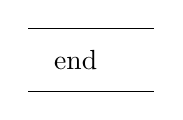
\begin{tikzpicture}[baseline=10,scale=0.8]
    \draw (0,0) -- (2,0);
    \draw (0,1) -- (2,1);
    %\vertbar[](0.5,0,1);
    \node[left] at (1.25, 0.5) {end};
    \vertbar[](1.5,1,0);
    \end{tikzpicture} \quad $\stackrel{\sim}{\longleftrightarrow}$ \quad
    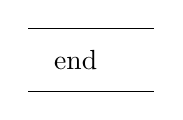
\begin{tikzpicture}[baseline=10,scale=0.8]
    \draw (0,0) -- (2,0);
    \draw (0,1) -- (2,1);
    %\vertbar[](0.5,1,0);
    \node[left] at (1.25, 0.5) {end};
    \vertbar[](1.5,0,1);
    \end{tikzpicture} \quad\quad \& \quad \quad     \begin{tikzpicture}[baseline=10,scale=0.8]
    \draw (0,0) -- (2,0);
    \draw (0,1) -- (2,1);
    \vertbar[](0.5,0,1);
    \vertbar[](1.5,1,0);
    \end{tikzpicture} \quad $\stackrel{\mu}{\longleftrightarrow}$ \quad
    \begin{tikzpicture}[baseline=10,scale=0.8]
    \draw (0,0) -- (2,0);
    \draw (0,1) -- (2,1);
    \vertbar[](0.5,1,0);
    \vertbar[](1.5,0,1);
    \end{tikzpicture}
     \caption{(Left) An instance of a reflection move. Under a reflection move, the quivers of the corresponding double plabic fences remain identical. (Right) A square move, the quivers of the corresponding double plabic fences undergo a quiver mutation at the vertex associated to the square face of the plabic fence where the move is applied.}
    \label{fig:reduction_and_sq_move}
\end{figure}

%%%%%%%%%%%%%%%%%%%%%%%%%%%%%%%%%%%%%%%%%%%%%%%%%%%%%%%%%%%%%%%%%%%%%
%%%%%%%%%%%%%%%%%%%%%%%%%%%%%%%%%%%%%%%%%%%%%%%%%%%%%%%%%%%%%%%%%%%%%
\subsection{Proof of Main Theorem} Let $D$ be a malleable divide. By \Cref{lem:malleable_to_plabic_fence}.(i), its quiver $Q(D)$ is mutation equivalent to the quiver of a plabic fence $\bG(D)$:
\begin{equation}\label{eq:proof_mutation_classes}
[Q(D)]=[Q(\bG(D))]
\end{equation}

By \Cref{cor:unique_dilation_mutation_equivalent_plabic_fence}.$(i)\&(ii)$, $Q(D)$ admits a unique non-degenerate potential $W(D)$, up to right equivalence, and a unique dilation $\delta(D)\in\Gclass[Q(D),W(D)]$. By \Cref{cor:unique_dilation_mutation_equivalent_plabic_fence}.$(iii)$, the cokernel module
    $$\coker\Eul_{(Q(D),W(D),\delta(D))}(t)\in\Z[t,t^{-1}]\mbox{-mod}$$
    is an invariant of the quiver mutation class $[Q(D)]$. By using \Cref{prop:P}.(ii) and \Cref{thm:unique-fence-G1}, we can endow the quiver $Q(\bG(D))$ with its unique non-degenerate potential $W(\bG(D))$, up to right equivalence, and its unique dilation $\delta(\bG(D))$. Then \eqref{eq:proof_mutation_classes} implies the isomorphism
    \begin{equation}\label{eq:determinants_equal_divide_fence}
    \coker\Eul_{(Q(D),W(D),\delta(D))}(t)\cong\coker\Eul_{(Q(\bG(D)),W(\bG(D)),\delta(\bG(D)))}(t)
    \end{equation}
    of $\Lambda$-modules. By \Cref{prop:dil_module_is_Alexander}, the right hand side of \eqref{eq:determinants_equal_divide_fence} equals the Alexander module $A_{L(\bG(D))}$ of $L(\bG(D))$. By \Cref{lem:malleable_to_plabic_fence}.(ii), $L(\bG(D))$ is smoothly isotopic to $L(D)$ and thus we have the following sequence of isomorphisms of $\Lambda$-modules:
    $$\coker\Eul_{(Q(D),W(D),\delta(D))}(t)\cong\coker\Eul_{(Q(\bG(D)),W(\bG(D)),\delta(\bG(D)))}(t)\cong A_{L(\bG(D))}\cong A_{L(D)},$$
    where the key isomorphism in the middle is \eqref{eq:coker_module_is_Alexander_algebraic} in \Cref{cor:cokernel_module_is_Alexander_algebraic_links}. This shows that the Alexander module $A_{L(D)}(t)$ of the link $L(D)$ of the divide $D$ can be entirely recovered from the quiver mutation class $[Q(D)]$. By \eqref{eq:alexander_module_monodromy}, the Alexander module $A_{L(D)}(t)$ is isomorphic to the integral monodromy module of the singularity. Therefore, the mutation class $[Q(D)]$ recovers the integral monodromy module of the singularity.\hfill$\Box$
    
%%%%%%%%%%%%%%%%%%%%%%%%%%%%%%%%%%%%%%%%%%%%%%%%%%%%%%%%%%%%%%%%%%%%%
%%%%%%%%%%%%%%%%%%%%%%%%%%%%%%%%%%%%%%%%%%%%%%%%%%%%%%%%%%%%%%%%%%%%%
\subsection{An explicit non-degenerate graded QP for divides} Even if it is not logically needed to conclude the Main Theorem, given a divide $D$ it can be useful to explicitly describe a representative for a non-degenerate potential $W(D)$ and compatible arrow-grading $d(D):Q(D)_1\lr\Z$, so that $W(D)$ is homogeneous of degree one. For that, recall from \cite[Definition 4.2]{FPST} that the vertices of $Q(D)$ are partitioned into three classes
\[
 Q(D)_0=V_{\ominus}(D)\sqcup V_{\bullet}(D)\sqcup V_{\oplus}(D),
\]
where $V_\ominus(D)$ denotes vertices labeled by $\ominus$ in \cite[Definition 4.2]{FPST}, $V_{\bullet}(D)$ is the set of vertices labeled by $\bullet$, and $V_\oplus(D)$ consists of the vertices labeled by $\oplus$. Consider the arrows in $Q(D)$ coming from the $\mbox{A}\Gamma$-diagram of $D$, which are pointing according to $\bullet\to\oplus\to\ominus\to\bullet$. Now, the potential and corresponding grading can be described as follows:\\

\begin{enumerate}

    \item {\it Potential $W(D)$}. First, one can equivalently describe $W(D)$ directly from $D$ and $Q(D)$. Indeed, by construction $Q(D)\sse\R^2$ can be considered as embedded in the plane where the divide is drawn. Then, the monomials contributing to the potential $W(D)$ are exactly the monomials coming from all the (planar) cycles of the quiver, i.e.~the bounded faces of the complement of the (graph underlying the) quiver. The monomials associated to cycles whose orientation coincides with the planar orientation contribute to $W(D)$ with a plus sign, and the others with a minus.\\

 \noindent   Alternatively, one can equivalently describe $W(D)$ by considering the plabic graph corresponding to $D$, via \cite[Definition 6.11]{FPST}. Then $W(D)$ can be declared to be the standard triangle potential associated to such plabic graph. See \cite[Definition 2.4]{Pressland19} or \cite[Remark 3.6]{BKM13} for the definition of potentials for (reduced) plabic graphs.\\
    
    \item {\it Grading $d(D)$}. Given the QP $(Q(D),W(D))$, we can choose the following arrow-grading $d_D$:
    \begin{equation}\label{eq:canonical-divide-grading}
 d_D(a)=
 \begin{cases}
 0&\mbox{ if }a:V_\ominus(D)\to V_\bullet(D)
       \text{ or }a:V_\bullet(D)\to V_\oplus(D),\\
 1&\mbox{ if }a:V_\oplus(D)\to V_\ominus(D).
 \end{cases}
\end{equation}
Since each summand of $W(D)$ contains exactly one arrow of type
\(V_\oplus\to V_\ominus\), the potential $W(D)$ has degree one, as required.
\end{enumerate}

\begin{remark}
It can be verified that triangle moves in divides, and square moves in the corresponding plabic graphs, yield QP-mutations compatible with dilations, not just quiver mutations.\hfill$\Box$
\end{remark}